\documentclass{beamer}

\usetheme{default}
\setbeamertemplate{bibliography item}{}

\usepackage{url}
\usepackage{xfrac}
\usepackage{paralist}

\title{NBICS Technologies}
\author{Alexander Aksentyev}
\institute{National Research Nuclear University ``MEPhI''}
\date{}

\setbeamercovered{transparent}

\begin{document}
	\begin{frame}
		\titlepage
	\end{frame}

\section{Nano-technologies}

\begin{frame}
	\frametitle{Carbon allotropes}
	\begin{columns}
		\column{.4\textwidth}
		Allotropy is the property of some chemical elements to exist in several different geometries (known as \emph{allotropes}) in the same physical phase
		\column{.6\textwidth}
		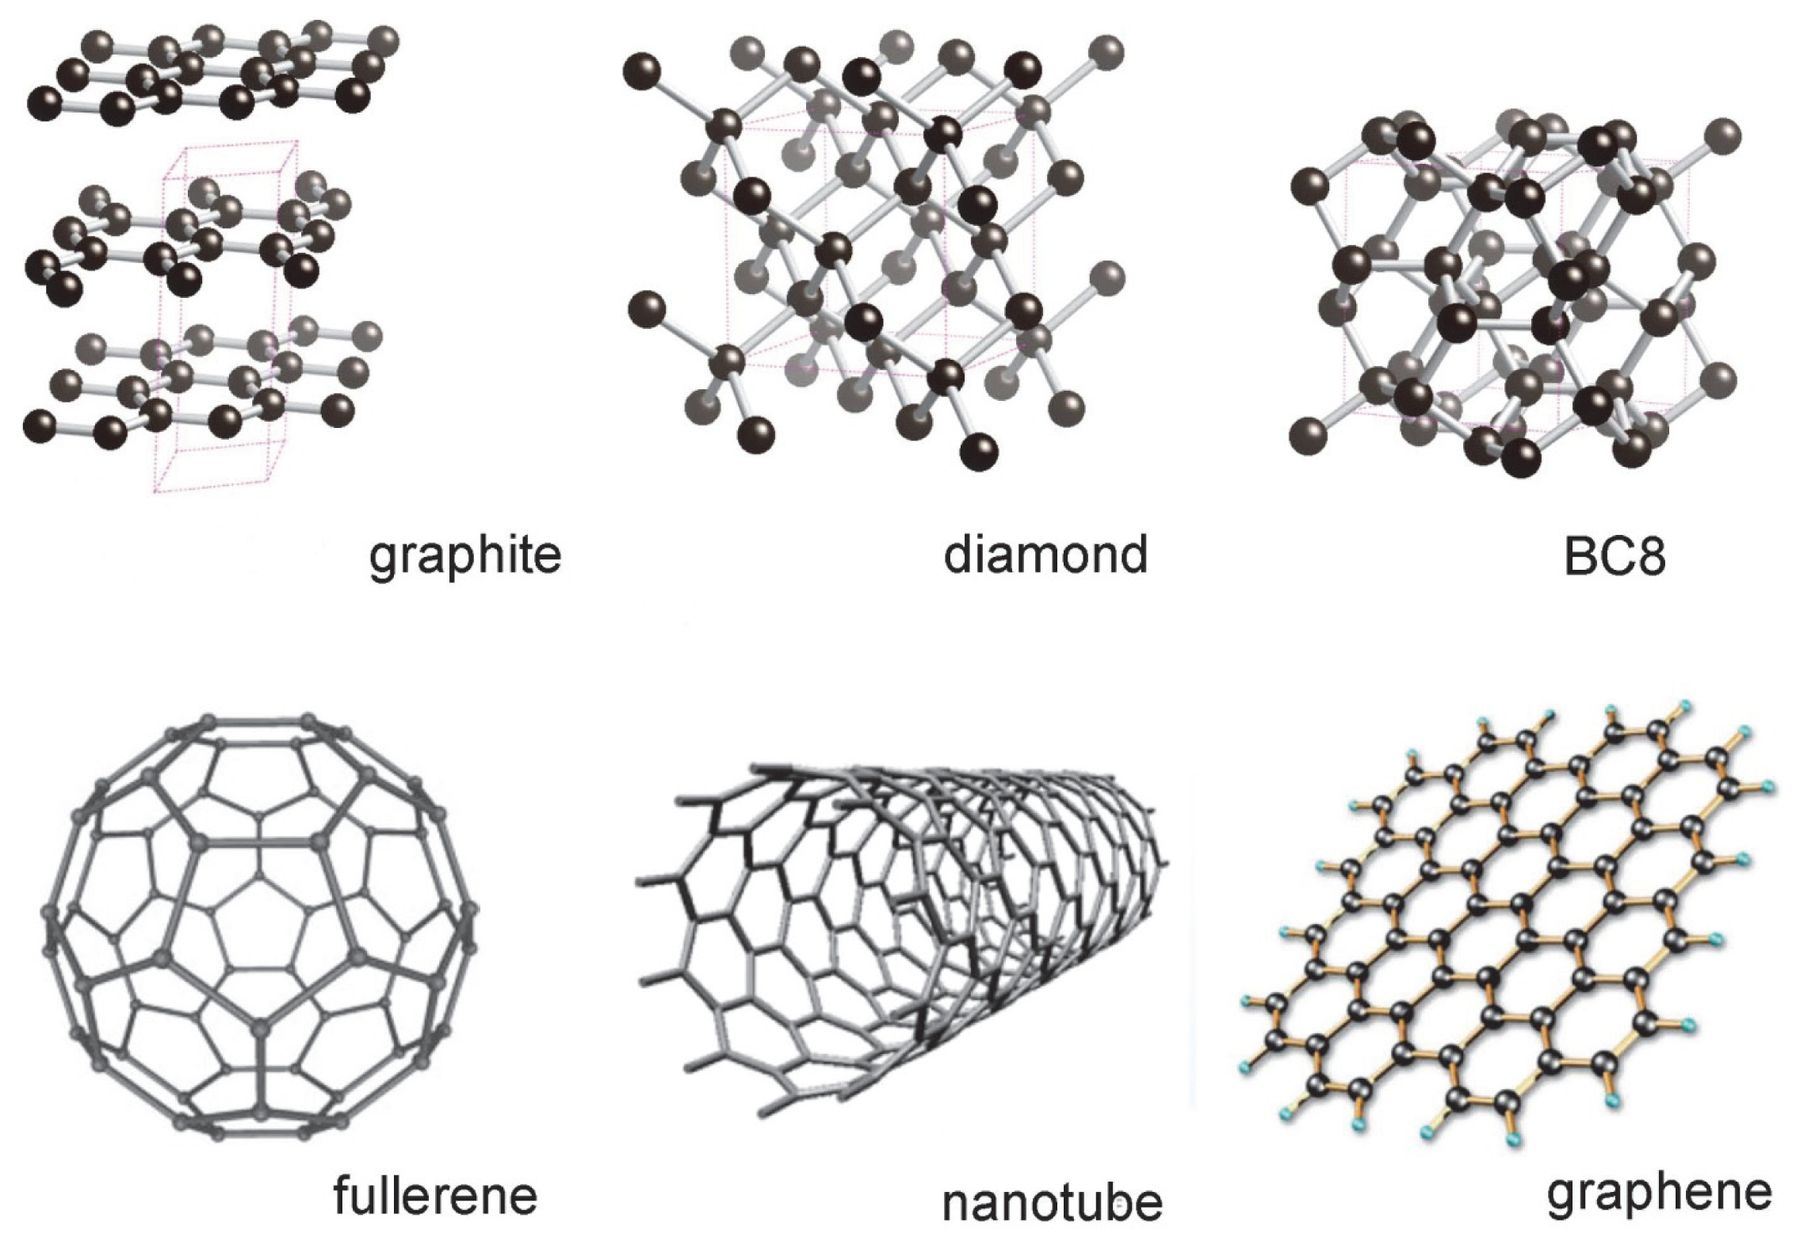
\includegraphics[scale=.45]{CarbAllotropes}
	\end{columns}
\end{frame}

\begin{frame}
	\frametitle{The Buckyball}
	\begin{columns}
		\column{.7\textwidth}
		\begin{itemize}
			\item The Buckminsterfullerene (named after inventor Richard Buckminster Fuller) was one of the first nanoparticles to be discovered (1985)
			
			\item Number of atoms: 20 to over 100; the most common type (C60) contains 60 carbon atoms
					
			\item Modifying a buckyball by adding or replacing an atom in order to change the properties of the buckyball is called \textbf{functionalization}
		\end{itemize}
		\column{.3\textwidth}
		\centering
		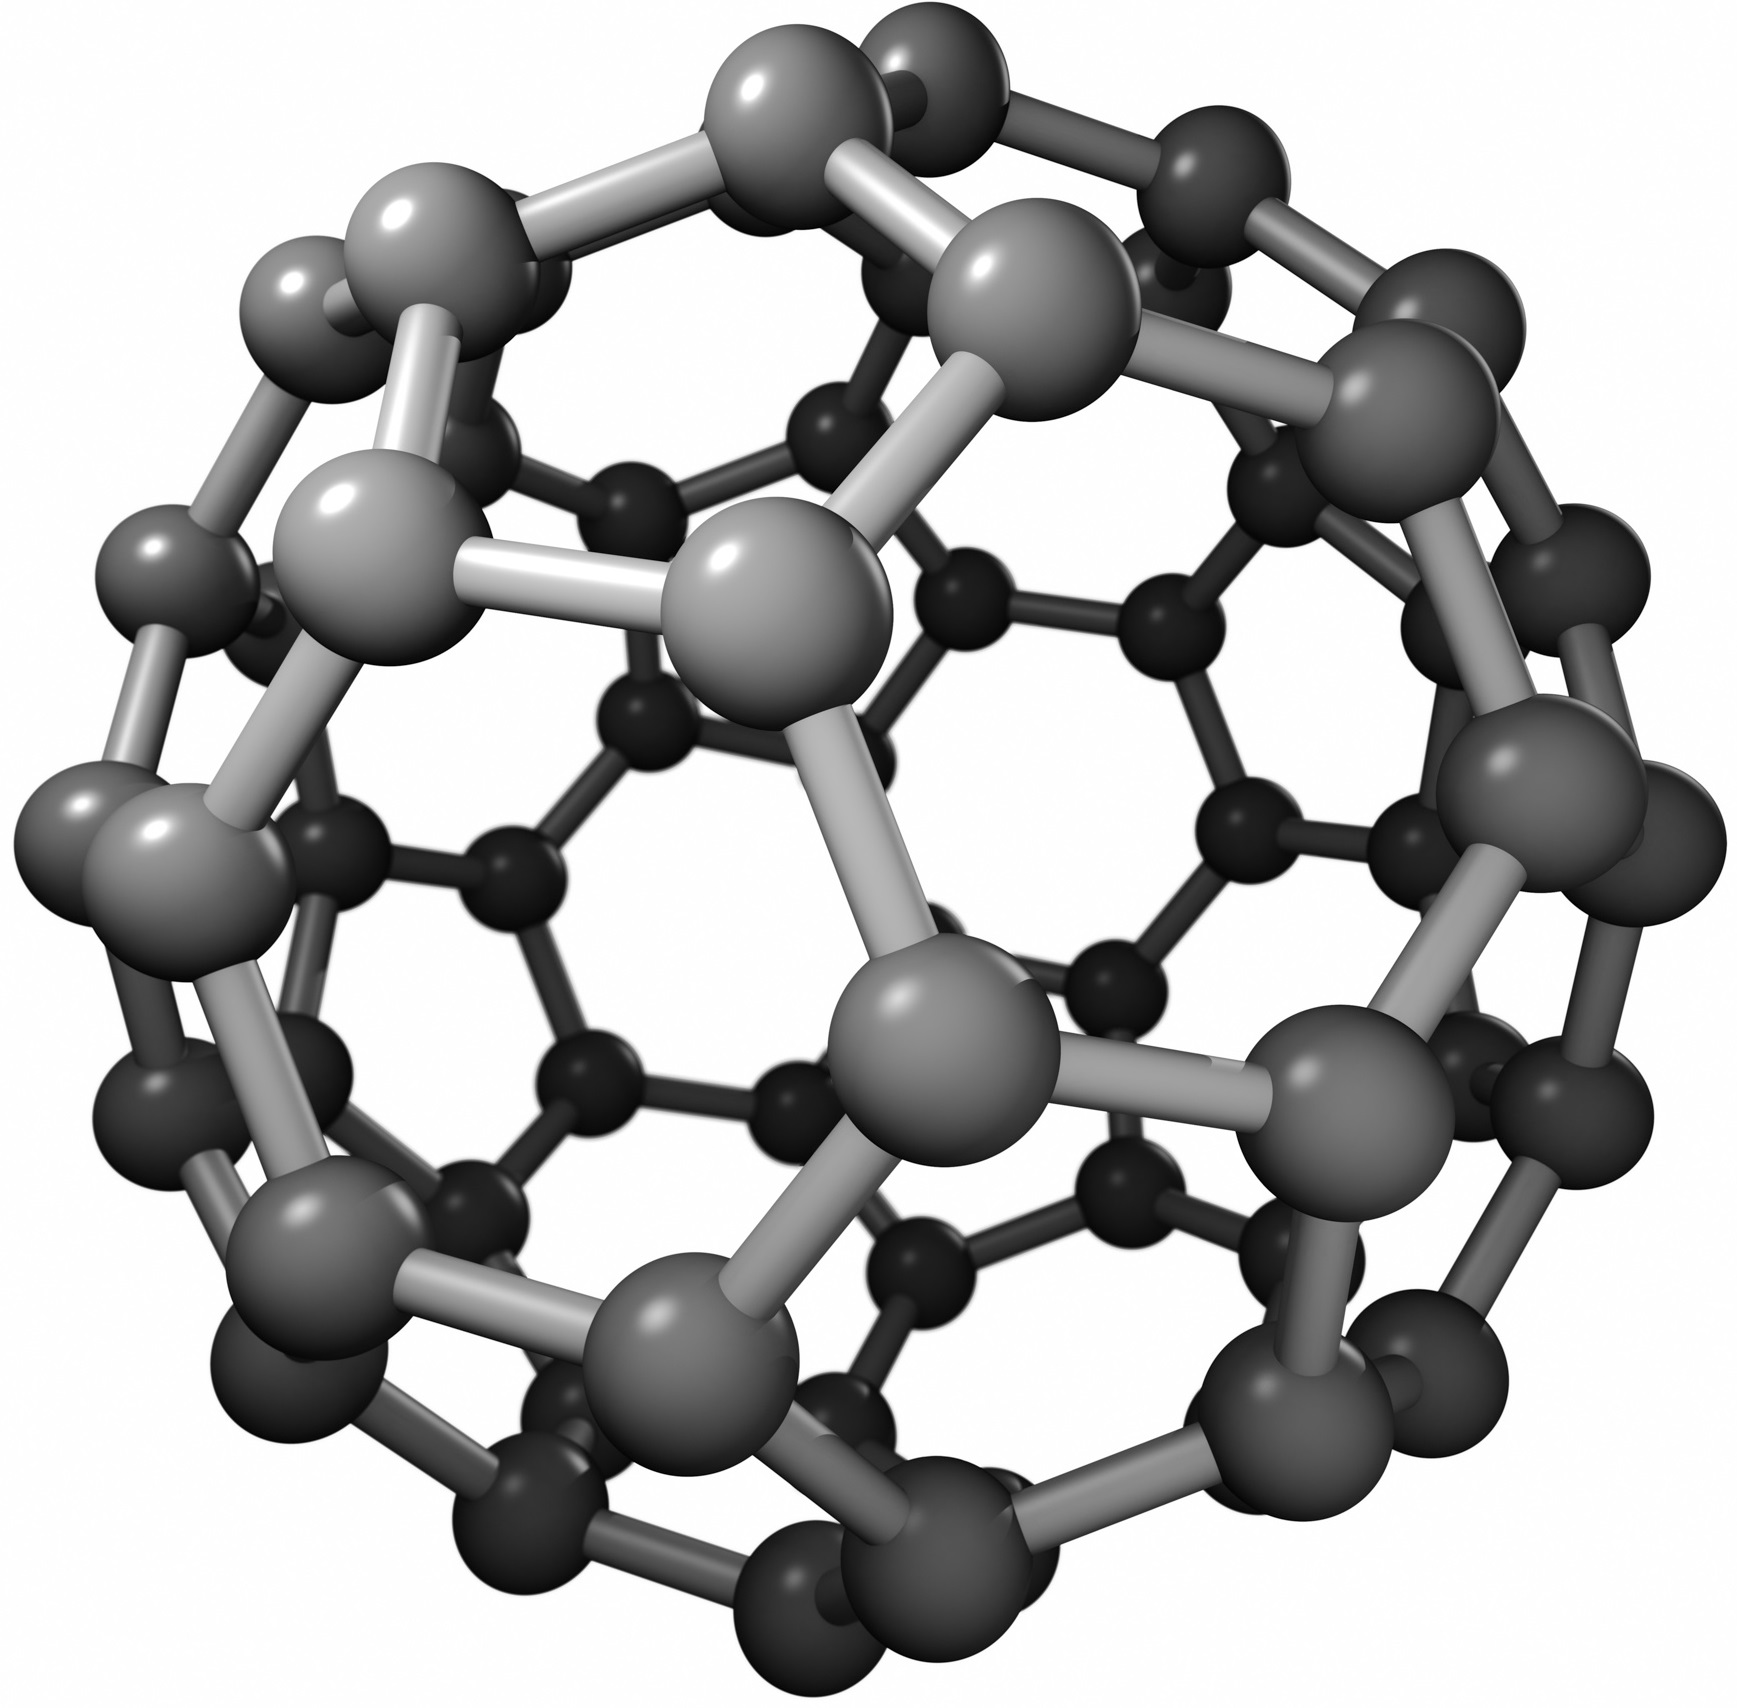
\includegraphics[scale=.2]{buckyball_white}
	\end{columns}
\end{frame}

\begin{frame}
	\frametitle{Uses}
	\begin{itemize}
		\item<1-> \textbf{Armor}. Hard as diamonds, buckyballs are potentially useful within armor
		
		\item<2-> \textbf{Medicine}. Functionalized buckyballs can be made soluble by body cells, and hence find the following medical applications:
			\begin{itemize}
				\item<2-> As antioxidants, because of their ability to absorb electrons in free radicals
				
				\item<2-> In targeted drug delivery. The buckyball encases a minute dose of a particular drug. By controlling the functionalization of the buckyball the drug is absorbed only by the necessary cells
			\end{itemize}
		\item<3-> \textbf{Fiber optics}. Because of their perfect spherical shape, buckyballs are able to transmit light
	\end{itemize}
\end{frame}

\begin{frame}
	\frametitle{The nanotube}
	\begin{columns}
		\column{.5\textwidth}
		\begin{itemize}
			\item Diameter $<$ 1 nm
			\item A few nano- up to a millimeter in length
			\item Symmetry: armchair, zig-zag, chiral
			\item Single/multiple wall CNTs
			\item Compared to steel:
				\begin{itemize}
					\item 100 $\times$ more difficult to tear apart
					\item 5 $\times$ as elastic
					\item a quarter density
				\end{itemize}
			\item High thermal conductivity
			\item Metallic/semi-conductive contingent on symmetry
		\end{itemize}
		\column{.65\textwidth}
		\begin{minipage}{.5\textheight}
			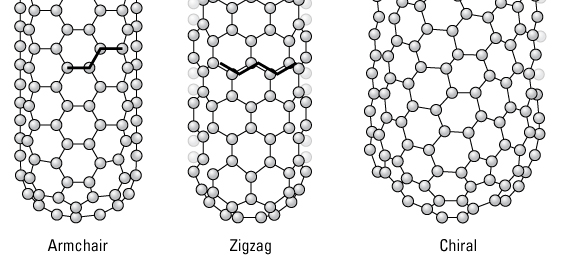
\includegraphics[scale=.65]{nanotube_orientations}
		\end{minipage}
	\begin{minipage}{.5\textheight}
		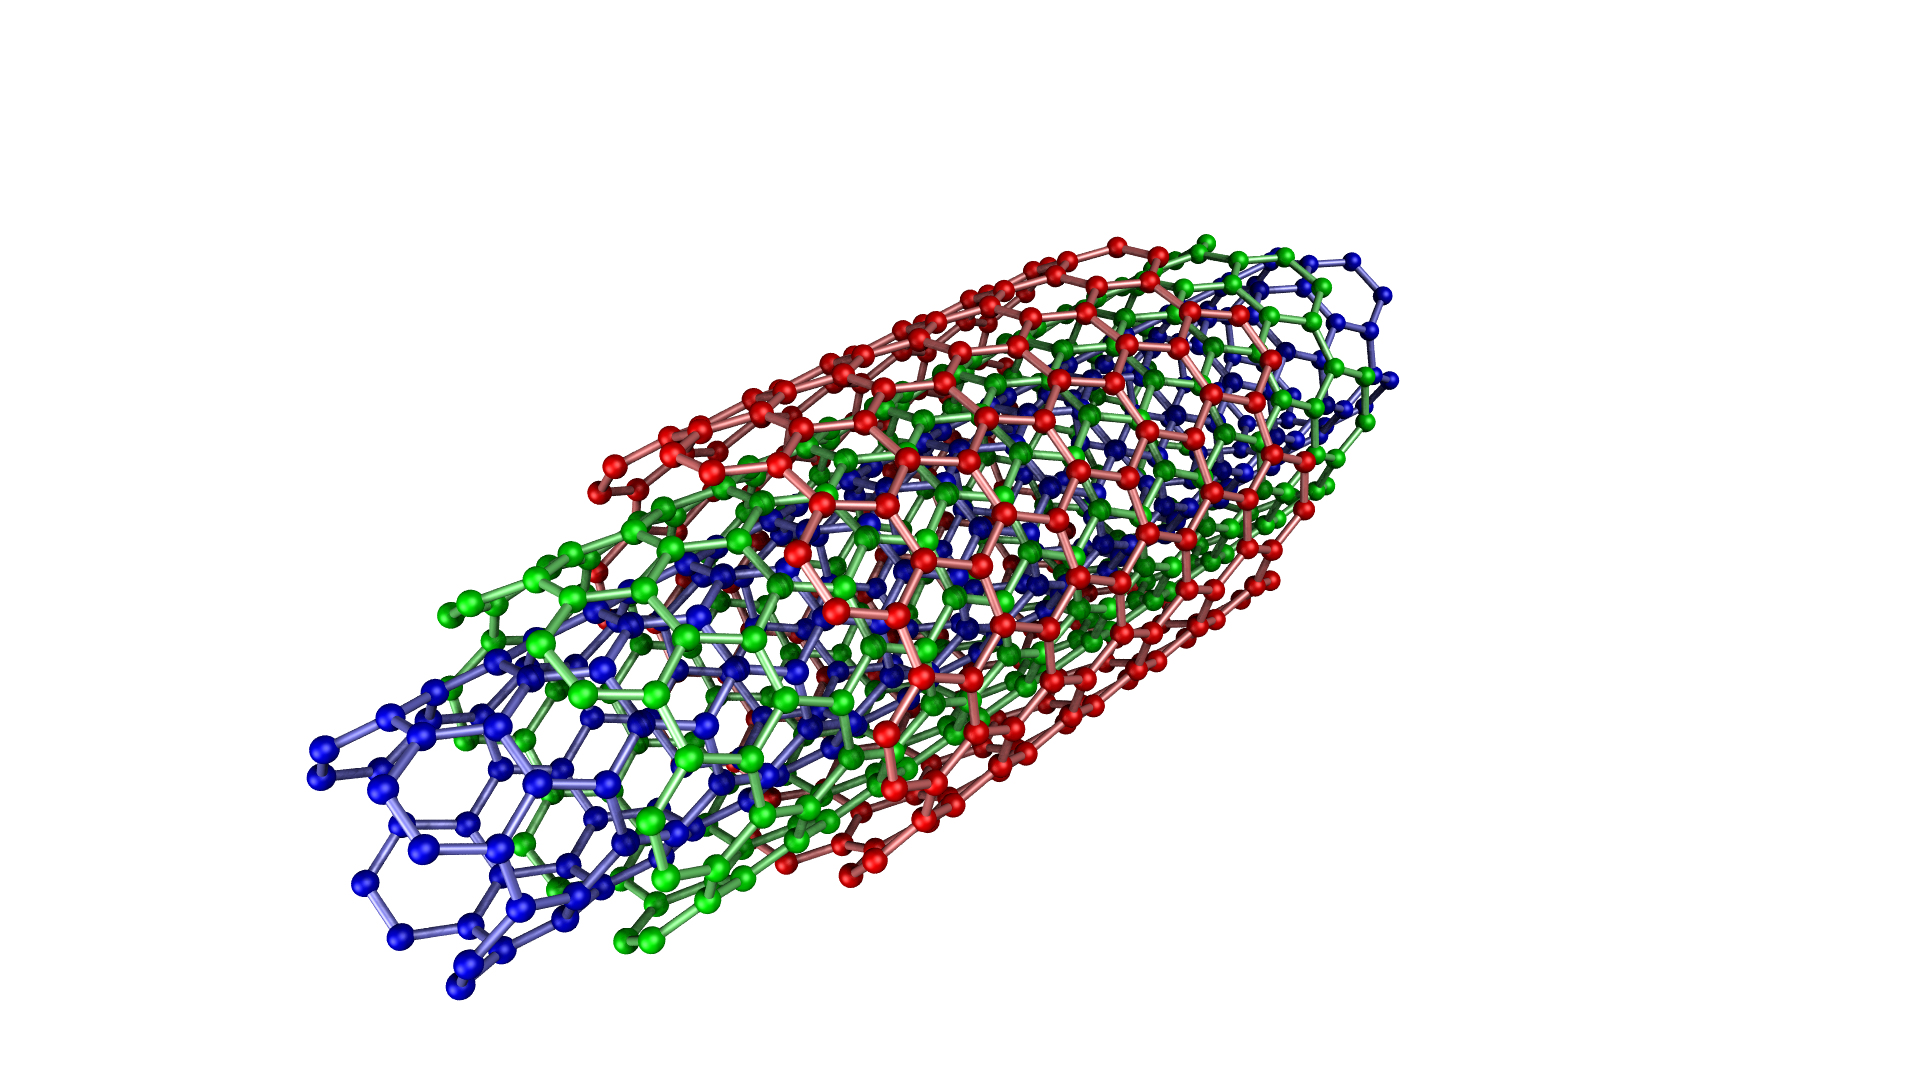
\includegraphics[scale=.1]{MWCNT}
	\end{minipage}
	\end{columns}
\end{frame}

\begin{frame}
	\frametitle{Uses}
	\begin{itemize}
	\item<1-> \textbf{Medicine}: functionalization, as well as their natural fluorescence, enable the use of CNTs as chemical sensors; they have also been shown to fuse well with bone, which could be used to diminish the implant rejection rate
	\item<2-> \textbf{Conductive plastics}: CNTs are the best known conductive fillers because of their high aspect ratio
	\item<3-> \textbf{Energy storage}: good battery electrodes due to high surface area ($\sim 1000$ m$^2$/g), good electrical conductivity, and linear geometry; the high surface area and thermal conductivity also make them useful as electrode catalysts in fuel cells
	\item<4-> \textbf{Molecular electronics}: their geometry, electrical conductivity, and the ability to be precisely derived, make CNTs invaluable connectors between switches at the nanoscale; their properties as semiconductors also make them usable as switches themselves
	\end{itemize}
\end{frame}

\begin{frame}
	\frametitle{The nanobud}
	\begin{columns}
		\column{.65\textwidth}
		\begin{itemize}
			\item A nanotube with a fullerene ball attached to it
			\item As chemically reactive as the fullerenes, as electrically conductive as the nanotubes
			\item The fullerene buds serve as additional anchors, modifying the mechanical properties of the whole structure
			\item Efficient field emitters, with the emission threshold 0.65 V/$\mu$m (a third of that of the nanotubes)
			\item Highly scalable production processes, therefore applications of industrial importance
		\end{itemize}
		\column{.5\textwidth}
			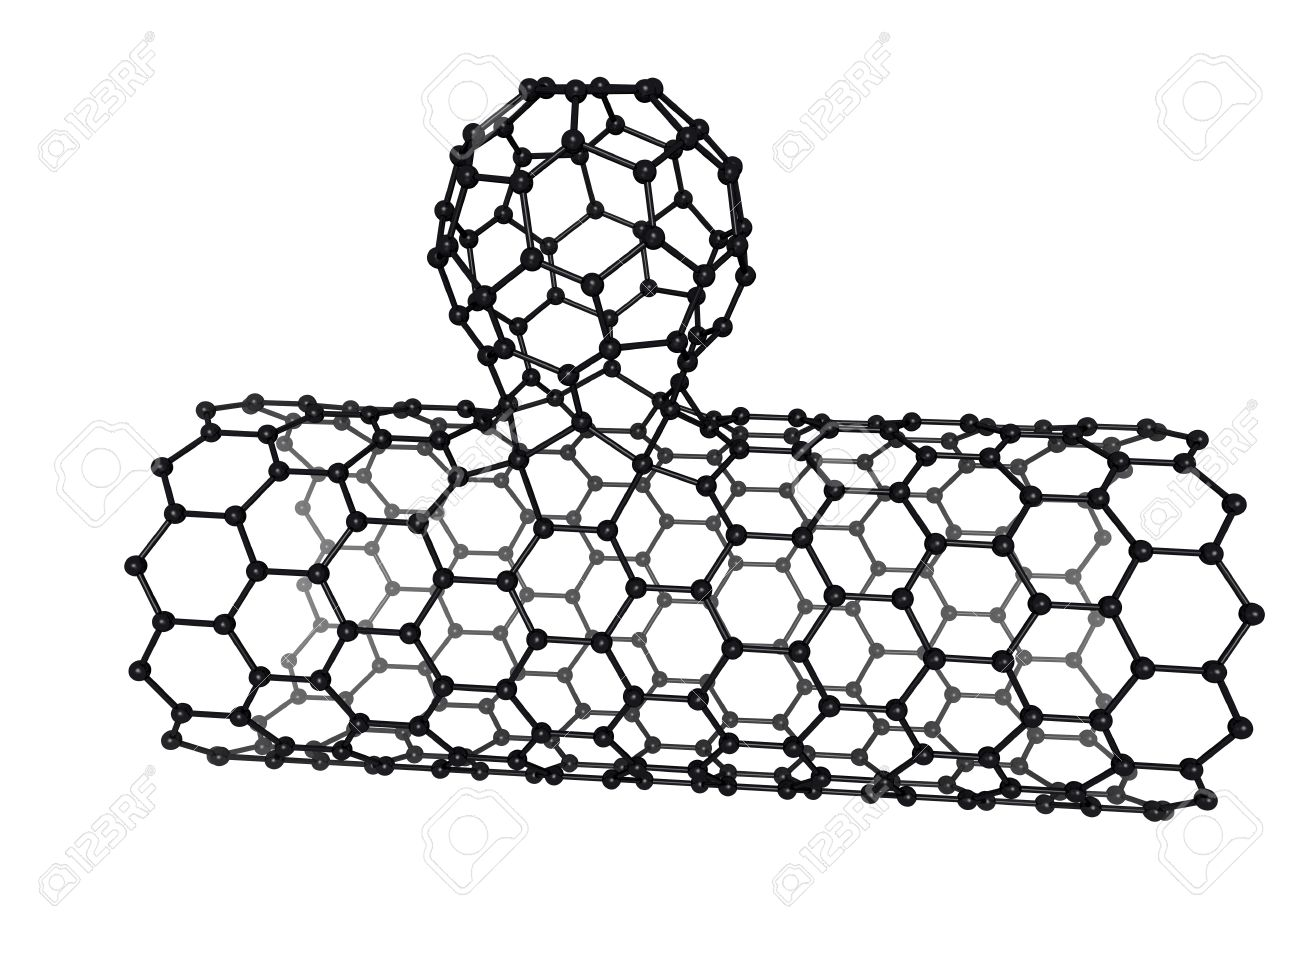
\includegraphics[scale=.15]{Nanobud}
	\end{columns}
\end{frame}

\section{Bio-technologies}
\begin{frame}
	\frametitle{Synthetic biology}
	\begin{center}
		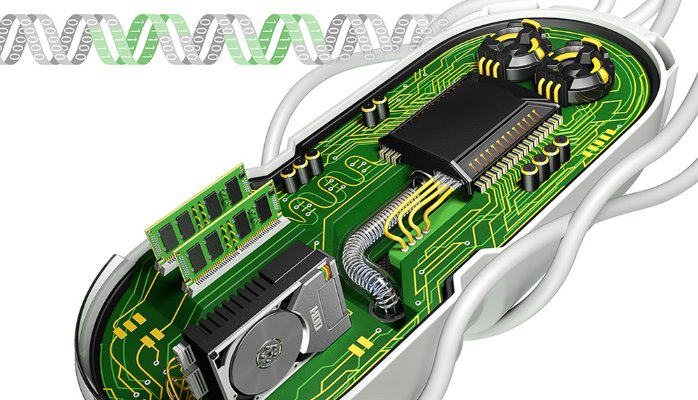
\includegraphics[scale=.4]{SynBio_main}
	\end{center}
	A set of technologies to construct living organisms with desired phenotypes
\end{frame}
\begin{frame}
		\begin{itemize}
		\item Systems biology studies complex biological systems as integrated wholes
		\item Synthetic biology studies how to build such systems for engineering applications
		\item Living systems provide a rich medium for controlling and processing
			\begin{itemize}
				\item information
				\item materials
				\item energy
			\end{itemize}
		\item Bacteria are the simplest known natural objects capable of replicating
	\end{itemize}
\end{frame}
\begin{frame}
	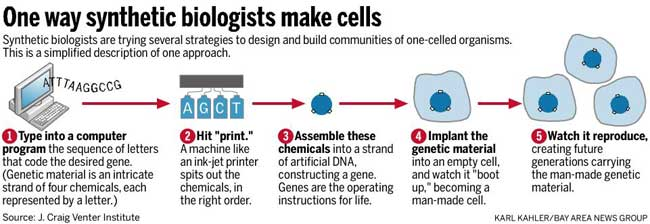
\includegraphics[scale=.5]{cell_synthesis}
	\\
	Enabling technologies:
	\begin{itemize}
		\item Standardization of DNA parts (BioBrick plasmids)
		\item DNA Synthesis
		\item DNA Sequencing
		\item Modular protein assembly
	\end{itemize}
\end{frame}
\begin{frame}
	\frametitle{Uses}
	
	\begin{itemize}
		\item<1-> \textbf{Materials}.  DNA synthesis and DNA sequencing have enabled the construction of microorganisms with specially engineered metabolic cycles. This is used in a variety of production processes: BioIsoprene, BioAcrylic, ``Green Chemicals''
		\item<2-> \textbf{Vaccines}. Bio Technologies provide tools to formulate vaccines via molecular engineering and DNA sequencing
		\item<3-> \textbf{Fuel}. Sugars from non-food biomass can be used to manufacture biofuels and renewable chemicals that are currently produced from expensive and price-volatile petroleum feedstocks
		\item<4-> \textbf{Waste disposal}. Bioplastics made from fermented sugars can be biodegraded by microbes already existing in soil and water environments
	\end{itemize}
\end{frame}

\section{Info-technologies}
\begin{frame}
	\begin{center}
		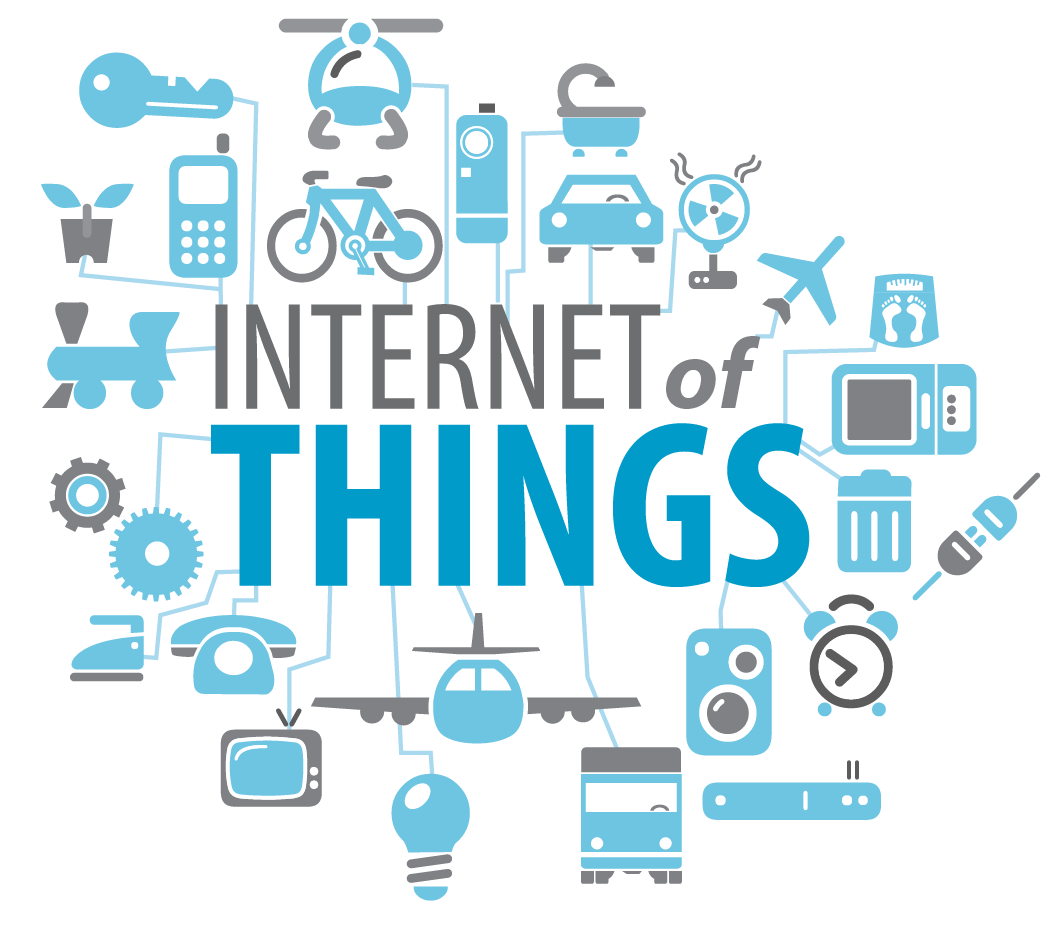
\includegraphics[scale=.5]{Internet_of_Things}
	\end{center}
\end{frame}
\begin{frame}
	\begin{itemize}
		\item The internetworking of physical devices to allow collection and exchange of information
		\item An instance of the more general class of \emph{cyber-physical systems}:
		\begin{itemize}
			\item smart grids
			\item smart homes
			\item smart cities
			\item intelligent transportation
		\end{itemize}
		\item Made by equipping all physical objects with identifying devices
		\item By 2020 there expected to be 20 billion connected devices
		\item The Internet of Things will therefore depend on the adoption of IPv6 to accommodate for the large address space 
	\end{itemize}
\end{frame}
\begin{frame}
	\frametitle{Enabling technologies}
	Some of the top 10 IoT-enabling technologies Gartner (IT research and advisory firm) identifies as most in-demand in 2017--2018:\\
	\begin{itemize}
		\item \textbf{IoT security}: IoT devices are open to both information and physical attacks, and many of them lack the processors and OS to afford sophisticated security approaches 
		\item \textbf{IoT analytics}: IoT business models require new algorithms, data structures, machine learning approaches to profit from the data that will become available
		\item \textbf{IoT device management}: as the devices comprising the IoT will find themselves in a variety of contexts, locations, physical states, the challenge is to develop data structures capable of learning and adapting to circumstances
	\end{itemize}
\end{frame}
\begin{frame}
	\begin{itemize}
		\item \textbf{IoT processors}: processor architecture defines the device capabilities, such as security, firmware updatability, ability to support device management agents, etc.
		\item \textbf{IoT OS}: traditional OS consume too much power, need fast processors, lack guaranteed real-time response, require too much memory. A range of specialized IoT OS has been developing
		\item \textbf{Event stream processing}: distributed stream computing platforms (DSCPs) have emerged to address the need to analyze the extremely high data rates generated by some IoT applications (telecom, telemetry) on-line 
		\item \textbf{IoT standards}: IoT devices need to interoperate, and IoT business models rely on sharing data between multiple devices and organizations
	\end{itemize}
\end{frame}
\begin{frame}
	\frametitle{Uses}
	The employment of the IoT leads to the following benefits:
	\begin{itemize}
		\item<2-> In manufacturing:
		\begin{itemize}
			\item<2->\textbf{Connected factory}: reduce downtime, increase productivity, maintain industry compliance
			\item<2-> \textbf{Connected machines}: optimize processes, improve overall equipment effectiveness, secure operations
			\item<2-> \textbf{Connected supply chain}: drive faster decision-making, reduce risk, improve supply chain visibility
		\end{itemize}
	\item<3-> In the energy field, \textbf{smart grids} enable pervasive monitoring and control of energy distribution networks to enhance energy delivery and reduce carbon emission
	\item<4-> In transportation:
	\begin{itemize}
		\item<4-> \textbf{on-line traffic analysis} improves logistics (smart infrastructure, smarter personal choices)
		\item<4-> \textbf{on-board wi-fi}, \textbf{real-time video}, \textbf{smart ticketing}, \textbf{centralized operations} enhance mass transit and passenger experience
	\end{itemize}
	\end{itemize}
\end{frame}


\section{Cogno-technologies}
\begin{frame}
	\frametitle{Neural interfaces}
	\begin{center}
		
\includegraphics[scale=.5]{Deus_ex_Adam_Jensen}
	\end{center}
\end{frame}
\begin{frame}
	\begin{columns}
		\column{.5\textwidth}
		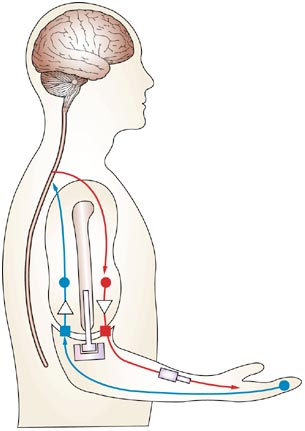
\includegraphics[scale=.55]{Neural_Interface_prosthetic}
		\column{.5\textwidth}
		\begin{itemize}
			\item A brain-computer interface (BCI) is a direct communication pathway between a wired brain and an external device
			\item Research and development are focused primarily on neuroprosthetics applications
			\item Was made possible by the development of \emph{electroencephalography} (EEG)
		\end{itemize}
	\end{columns}
\end{frame}
\begin{frame}
	\frametitle{Types of interfaces}
	\begin{columns}
		\column{.5\textwidth}
		\begin{itemize}
			\item EEG-based:
			\begin{itemize}
				\item Electrocorticography: electrodes embedded in a plastic pad are placed above the cortex, beneath the cranium
			\end{itemize}
			\item Non-EEG-based:
			\begin{itemize}
				\item Pupil-size oscillation: an eye's pupil contracts according to the brightness of the looked at object
			\end{itemize}
		\end{itemize}
		\column{.5\textwidth}
		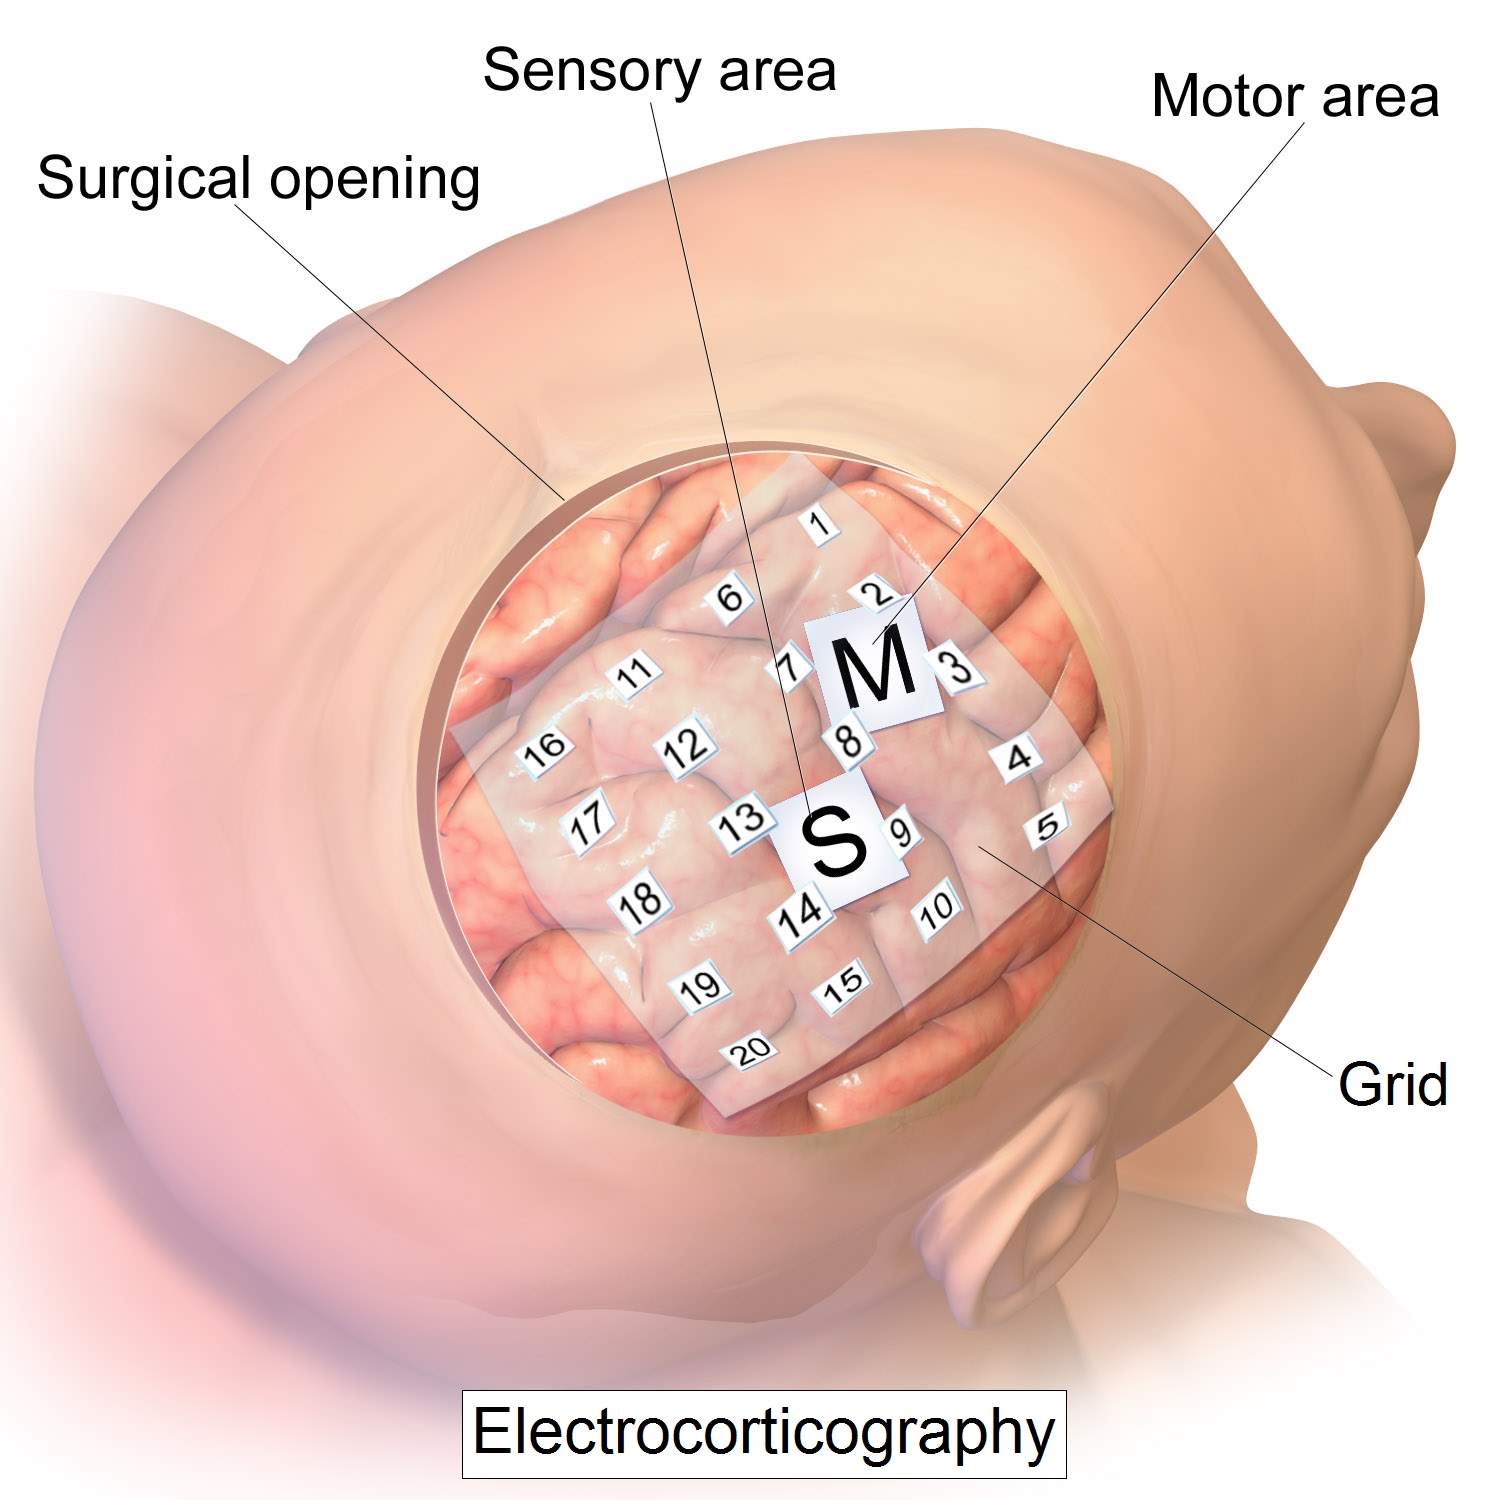
\includegraphics[scale=.15]{ECoG}
	\end{columns}
\end{frame}
\begin{frame}
	\frametitle{BCI applications}
	\begin{center}
		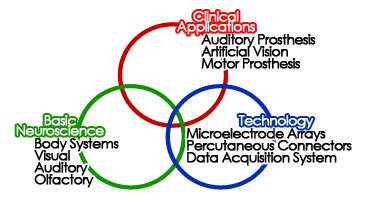
\includegraphics[scale=.8]{BCI_applications_Venn}
	\end{center}
\end{frame}

\section{Socio-technologies}
\begin{frame}
	\frametitle{Educational technology}
	\begin{columns}
		\column{.5\textwidth}
		
\includegraphics[scale=.5]{EdTech_main}
		\column{.5\textwidth}
		\begin{itemize}
			\item Learning theory
				\begin{itemize}
					\item Behaviorism
					\item Cognitivism
					\item Constructivism
				\end{itemize}
			\item Computer-based training
			\item Online learning
			\item Mobile learning
		\end{itemize}
	\end{columns}
\end{frame}

\begin{frame}
	\frametitle{Top technologies:\only<1>{ AI, VR, VW}\only<2>{ AR}\only<3>{ ARG}}
	
		\only<1>{
			\begin{description}[VW]
				\item[AI] Customized learning-experience is already a reality. An intelligent tutoring system consists of:
					\begin{description}[tutoring model]
						\item[learner model] to assess how the student is doing 
						\item[tutoring model] to determine what material to present next 
						\item[domain model] to represent it appropriately
					\end{description}
				\item[VR] Learn by doing. One can now explore and interact with molecules and galaxies, thanks to virtual reality
				\item[VW] Socialization is a vital part in a person's development, and as it turns out, introverted kids don't feel anxious interacting online
			\end{description}
		}
	
		\only<2>{Use the user's context to specify information}
		\only<2>{
			\begin{center}
				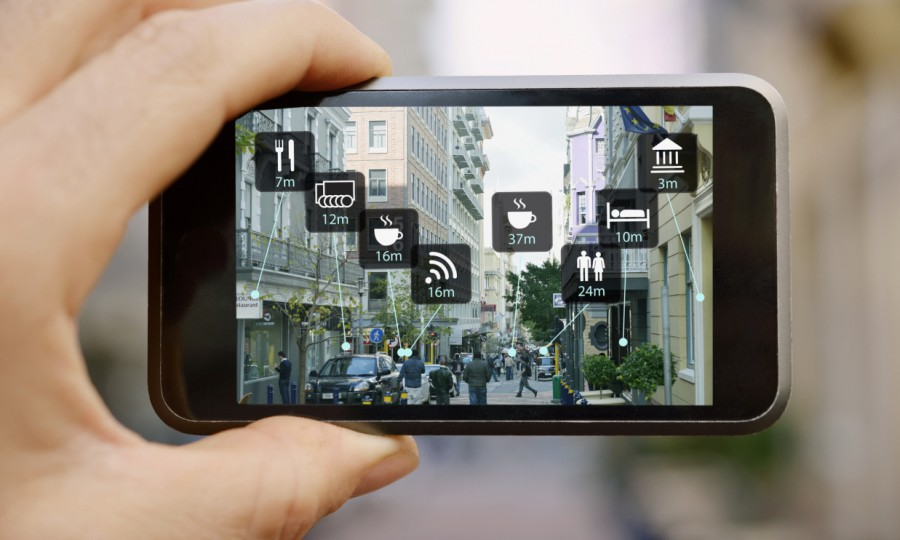
\includegraphics[scale=.4]{AR_example}
			\end{center}
		}
		
		\only<3>{Enabling the use of communication tools typically used in the workspace, provides learning opportunities by situating important decisions in a thematic story}
		\only<3>{
			\begin{center}
				
\includegraphics[scale=.15]{ARG_example}
			\end{center}
		}
\end{frame}

\begin{frame}[allowframebreaks]
	\frametitle{References}
	\nocite{*}
	\bibliographystyle{plain}
	\bibliography{Presentation}
\end{frame}

\end{document}